%%%%%%%%%%%%%%%%%%%%%%%%%%%%%%%%%%%%%%%%%
% Short Sectioned Assignment
% LaTeX Template
% Version 1.0 (5/5/12)
%
% This template has been downloaded from:
% http://www.LaTeXTemplates.com
%
% Original author:
% Frits Wenneker (http://www.howtotex.com)
%
% License:
% CC BY-NC-SA 3.0 (http://creativecommons.org/licenses/by-nc-sa/3.0/)
%
%%%%%%%%%%%%%%%%%%%%%%%%%%%%%%%%%%%%%%%%%

%----------------------------------------------------------------------------------------
%	PACKAGES AND OTHER DOCUMENT CONFIGURATIONS
%----------------------------------------------------------------------------------------

\documentclass[letterpaper, fontsize=11pt]{scrartcl} % A4 paper and 11pt font size

\usepackage[T1]{fontenc} % Use 8-bit encoding that has 256 glyphs
\usepackage{fourier} % Use the Adobe Utopia font for the document - comment this line to return to the LaTeX default
\usepackage[english]{babel} % English language/hyphenation
\usepackage{amsmath,amsfonts,amsthm} % Math packages

\usepackage{lipsum} % Used for inserting dummy 'Lorem ipsum' text into the template
\usepackage[margin=1in]{geometry} %set margins -TA
\usepackage{sectsty} % Allows customizing section commands
\allsectionsfont{\centering \normalfont\scshape} % Make all sections centered, the default font and small caps
\usepackage{enumitem}
\usepackage{fancyhdr} % Custom headers and footers
\usepackage{graphicx}
\pagestyle{fancyplain} % Makes all pages in the document conform to the custom headers and footers
\fancyhead{} % No page header - if you want one, create it in the same way as the footers below
\fancyfoot[L]{\textit{CME 102 Winter '17-'18}} % Empty left footer
\fancyfoot[C]{} % Empty center footer
\fancyfoot[R]{Tim Anderson} % Page numbering for right footer
\renewcommand{\headrulewidth}{0pt} % Remove header underlines
\renewcommand{\footrulewidth}{0pt} % Remove footer underlines
\setlength{\headheight}{14pt} % Customize the height of the header


\usepackage{mdframed}
\usepackage{caption}
\usepackage{subcaption}
\usepackage{float}
\usepackage{array}
\usepackage{soul}
\usepackage{amsmath}
\usepackage{graphicx} % Required to insert images
\usepackage{multicol}
\usepackage{enumitem}
\usepackage{amssymb}
\usepackage{bm}
\usepackage{verbatim}
\usepackage{hyperref}

\allowdisplaybreaks

\numberwithin{equation}{section} % Number equations within sections (i.e. 1.1, 1.2, 2.1, 2.2 instead of 1, 2, 3, 4)
\numberwithin{figure}{section} % Number figures within sections (i.e. 1.1, 1.2, 2.1, 2.2 instead of 1, 2, 3, 4)
\numberwithin{table}{section} % Number tables within sections (i.e. 1.1, 1.2, 2.1, 2.2 instead of 1, 2, 3, 4)

\setlength\parindent{0pt} % Removes all indentation from paragraphs - comment this line for an assignment with lots of text
\begin{document}

%----------------------------------------------------------------------------------------
%	TITLE SECTION
%----------------------------------------------------------------------------------------

\newcommand{\horrule}[1]{\rule{\linewidth}{#1}} % Create horizontal rule command with 1 argument of height

%----------------------------------------------------------------------------------------
%	PROBLEM 1
%----------------------------------------------------------------------------------------

\section*{Laplace Transform Review Problems}

\begin{enumerate}
\item Find the Laplace transform for the following functions. If an image is given, first write out the function and then take the transform.

\begin{enumerate}

\item $e^{-t}\sinh (4t)$

\item $1.5\sin(3t-\pi/2)$

\item Function given in the following figure:
\begin{figure}[H]
\centering 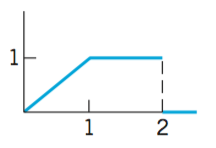
\includegraphics[width = 0.3\columnwidth]{LaplaceFig1.png}
\end{figure}
\end{enumerate}

\item Solve the following initial value problems:
\begin{enumerate}
\item $y'' + 9y = 10e^{-t},\quad y(0) = y'(0) = 0$

\item $y'' + 0.04y = 0.02t^2,\quad y(0) = -25,\quad y'(0) = 0$
\end{enumerate}

\item Find the inverse Laplace transform:
\begin{enumerate}
%Kreyszig 6.3 #16
\item $Y(s) = \frac{2(e^{-s} - e^{-3s})}{s^2 - 4}$

%Kreyszig 6.3 #17
\item $Y(s) = \frac{1 + e^{2\pi(s+1)}(s +1)}{(s + 1)^2 + 1}$
\end{enumerate}

%Kreyszig 6.3 #21
\item Solve the initial value problem: $$y'' + 9y = f(t),\quad y(0) = 0,\quad y'(0) = 4$$ where $f(t) = 8\sin(t)$ for $0 < t < \pi$ and 0 for $t > \pi$.

%Kreyszig 6.4 #6
\item Solve the initial value problem:
$$y'' + 4y' + 5y = \delta(t-1),\quad y(0) = 0,\quad y'(0) = 3$$

\item 
\begin{enumerate}
%Kreyszig 6.6 #3
\item Find the Laplace transform: $f(t) = \frac{1}{2}te^{-3t}$

\item Find the inverse Laplace transform: $F(s) =\cot^{-1}\left(\frac{s}{\pi}\right)$. \textit{Hint:} $\frac{d}{dx}\left(\cot^{-1}(x)\right) = \frac{-1}{1 + x^2}$.

\end{enumerate}

\item Solve $y'' + 4y = f(t),\quad y(0) = y'(0) = 0$ with $f(t)$ defined by the following figure:
\begin{figure}[H]
\centering 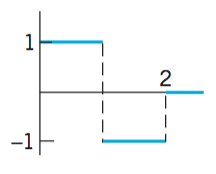
\includegraphics[width = 0.3\columnwidth]{LaplaceFig2.png}
\end{figure}

\end{enumerate}



%----------------------------------------------------------------------------------------





\end{document}